\documentclass[12pt]{article}

\usepackage{amsmath, amsfonts, bm, graphicx}
\usepackage{tabularx}
\usepackage{booktabs} 
\usepackage{float}

\title{Ph291E Lab 6 -- Physics with Python I: Plotting}
\author{
    Zeshui Song\\
    The Cooper Union
}
\date{September 25, 2025}

\begin{document}

\maketitle

\section{Purpose}  
In this lab, Python will be used to compute and plot the solutions to wave equations. In particular, interference patterns from Young's double slit experiment will be visualized along with the single slit and N-slit cases.
\newpage
\section{Results}
\paragraph{Double Slit}\mbox{}\\
\begin{figure}[H]
    \centering
    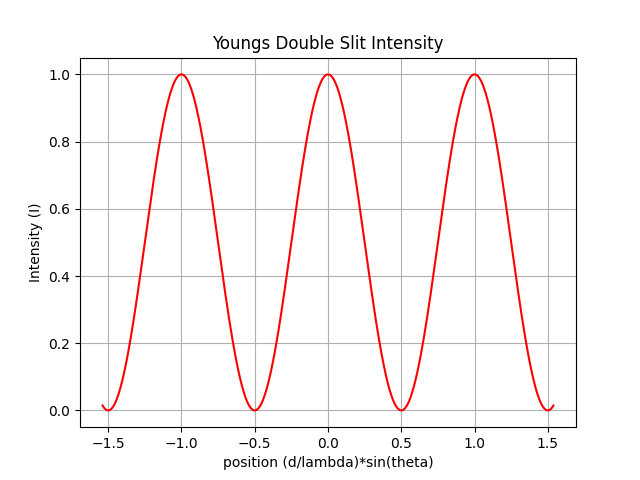
\includegraphics[width=0.8\textwidth]{youngs_ds.png}
\caption{Young's Double Slit Intensity Pattern ($d=1\,\mathrm{\mu m},\,\lambda=650\,\mathrm{nm}$) using the following linspace command: \texttt{theta = np.linspace(-np.pi/2.0, np.pi/2.0, int(np.pi/0.001))}}
\end{figure}
\paragraph{N-Slit} \mbox{}\\
\begin{figure}[H]
    \centering
    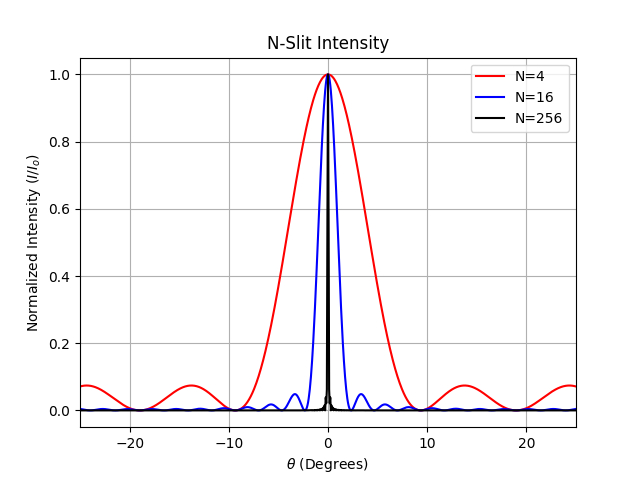
\includegraphics[width=0.8\textwidth]{N-Slit.png}
\caption{N-Slit Intensity Pattern with varying slits ($d=1\,\mathrm{\mu m},\,\lambda=650\,\mathrm{nm}$)}
\end{figure}

\section{Conclusion}
\section{Answers to Questions}
\end{document}
